%課題研究レジュメテンプレート ver. 1.2

\documentclass[uplatex]{jsarticle}
\usepackage[top=20mm,bottom=20mm,left=20mm,right=20mm]{geometry}
\usepackage[T1]{fontenc}
\usepackage{txfonts}
\usepackage{wrapfig}
\usepackage[expert,deluxe]{otf}
\usepackage[dvipdfmx,hiresbb]{graphicx}
\usepackage[dvipdfmx]{hyperref}
\usepackage{pxjahyper}
\usepackage{secdot}
\usepackage{here}

\makeatletter
  \renewcommand{\section}{%
    \if@slide\clearpage\fi
    \@startsection{section}{1}{\z@}%
    {\Cvs \@plus.5\Cdp \@minus.2\Cdp}% 前アキ
    {.5\Cvs \@plus.3\Cdp}% 後アキ
    %{\normalfont\Large\headfont\raggedright}}
    {\normalfont\raggedright}}

  \renewcommand{\subsection}{\@startsection{subsection}{2}{\z@}%
    {\Cvs \@plus.5\Cdp \@minus.2\Cdp}% 前アキ
    {.5\Cvs \@plus.3\Cdp}% 後アキ
    %{\normalfont\large\headfont}}
    {\normalfont}}

  \renewcommand{\subsubsection}{\@startsection{subsubsection}{3}{\z@}%
    {\Cvs \@plus.5\Cdp \@minus.2\Cdp}%
    {\z@}%
    %{\normalfont\normalsize\headfont}}
    {\normalfont}}
\makeatother
%ここから上を編集する必要はない.





\title{\vspace{-14mm}PBLを経験した学生の学習成果の測定}
\author{PMコース 矢吹研究室 1342015 板倉 啓太}
\date{}%日付を入れる必要はない.
\pagestyle{empty}%ページ番号は振らない.
\begin{document}
\maketitle





\section{研究の背景}

近年,情報系の分野における実践的な教育方法として,\cite{PBL}\cite{PBL1}PBLに対する注目度が高まっている。PBLとは,Project Based Learning(プロジェクト・ベースト・ラーニング)の略称であり,
「プロジェクト型学習」や「問題解決型授業」などと言われる.PBLは欧米発祥の教育手法であり,日本での医歯薬学の分野など実習・演習が重視される分野においては以前から有効な教育手法として知られてきた.PBLが,特にここ数年,情報系での分野の新しい教育手法として大きな注目を集め始めた.現在情報技術が多くの産業の基盤となり,情報技術 に関する高い技術力や活用力を有する人材がこれまで以上に強く求められるようになっている.その背景には,情報系分野における教育に対して,現在以上の実践性が必要だと考える強い問題意識の台頭である.こうした中で,高度な人材の育成に向けて,より実践的な教育を実現するための効果的な教育手法としてPBLが注目を集めているのである.

しかし実際のところ,PBLの実施方法に関する論文や書籍はまだ少ないため,PBLを実施している大学の多くは限られた情報の中で課題を設計・実施しているのが現状である.加えて,PBLは全ての参加者に対して有効的な教育ツールではなく,常に改善が求められている.また,PBLを取り入れた授業を受講した学生個人に対する評価は,グループ作業を基本としているため,特に個人に対する評価が困難である.そこで行動特性の定量的な評価をするために,\cite{ルーブリック評価}ルーブリック評価という手法がある.ルーブリック は,学習到達度を示す評価基準を観点と尺度からなる表として示したものである.

これらの点を踏まえ,ルーブリック評価の手法を用いてアンケート表を作成し,個人の学習到達状況を調査し今後の改善案を模索し提案する.




\section{研究の目的}

本研究では,プロジェクトマネジメント学科のソフトウェアコースのPM実験を受講した学生を対象に学習到達度を調査する.加えて,ここで調査した結果を基に,今後のPM実験における改善案を考察する.





\section{プロジェクトマネジメントとの関連}

PBLとはプロジェクト型学習とも呼ばれ,プロジェクトを通しての課題の解決を目標にした教育手法である.これはプロジェクトマネジメントの知識エリアにおいては主にプロジェクト統合マネジメントに該当する.加えてプロジェクト・コミュニケーション・マネジメントやプロジェクト・スコープ・マネジメントにも該当する.




\begin{wrapfigure}[8]{r}{8cm}
\vspace*{-\intextsep}
%\includegraphics[width=6,clip]{ファイル名}\label{参照用ラベル}
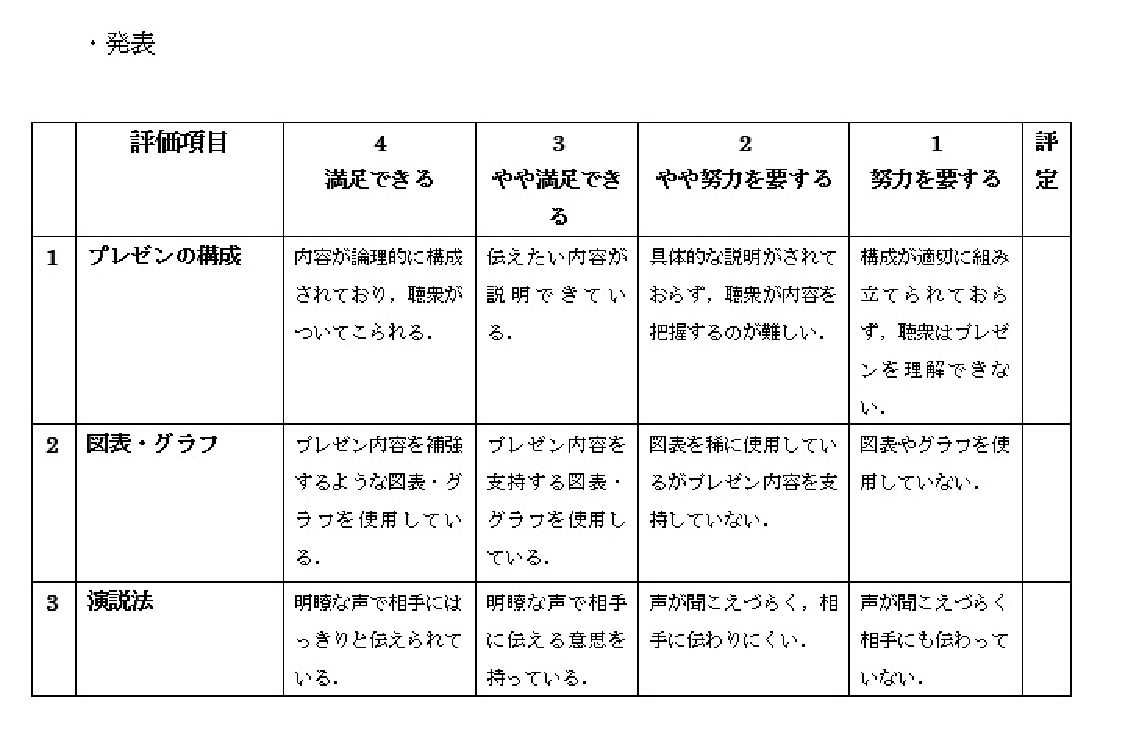
\includegraphics[width=8cm,clip]{g2.pdf}
\caption{ルーブリック表}\label{ルーブリック表}
\end{wrapfigure}



\section{研究の方法}

以下の順に研究を進める.

\begin{enumerate}
\item ソフトウェアコースのPM実験を受講した学生に対し4段階評価でのアンケート調査をする.
\item ルーブリック評価の手法を用いてアンケート項目ごとの定義を段階別に設定する.
\item アンケート結果を基に,PM実験を終えた学生の学習到達度をグラフ化し,今後の改善案を考察する.

\end{enumerate}


\begin{wrapfigure}[10]{r}{10cm}
\vspace*{-\intextsep}
%\includegraphics[width=6,clip]{ファイル名}\label{参照用ラベル}
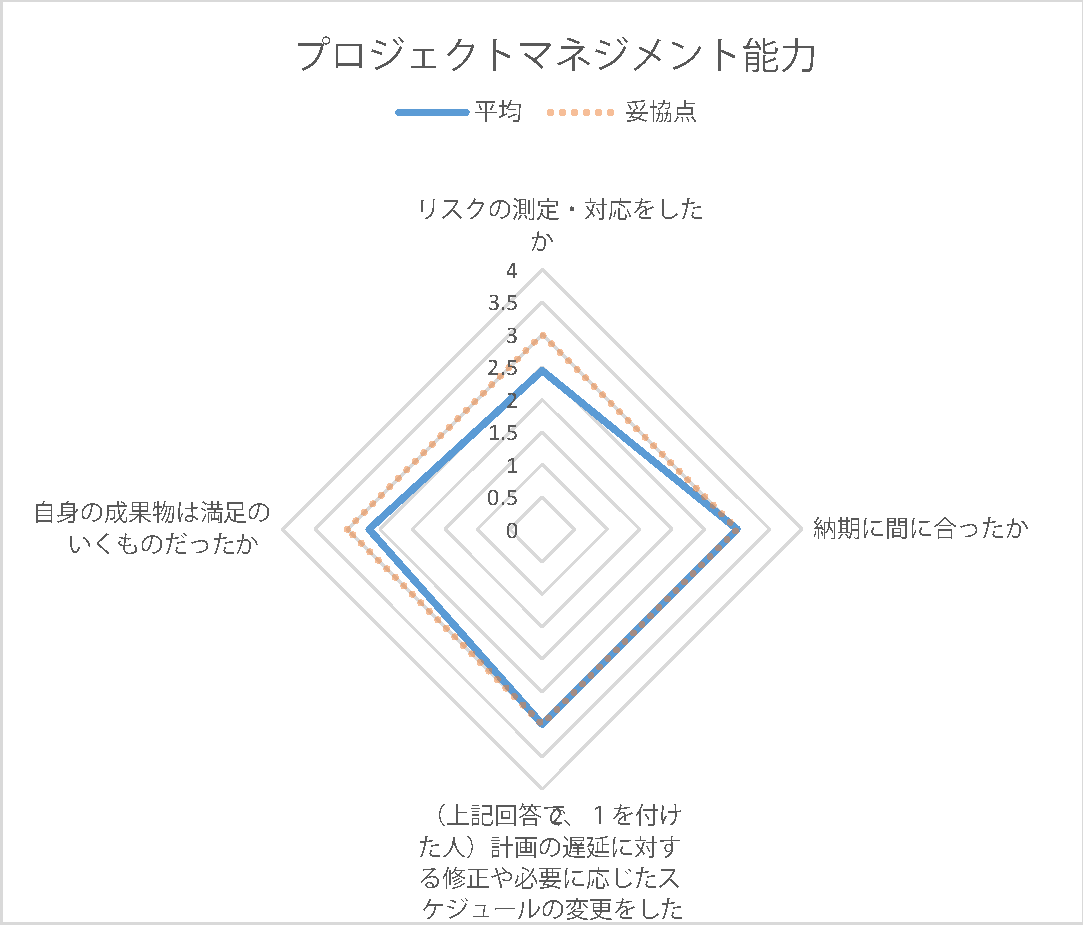
\includegraphics[width=10cm,clip]{g1.pdf}
\caption{アンケート結果}\label{アンケート結果}
\end{wrapfigure}



\section{現在の進捗状況}

上記の手順でPM実験のソフトウェアコースを学習し終えた学生の一部からアンケート調査を行った.結果は,最終的な納期には間に合っていたものの,プロジェクトを進行していく上で計画の遅延に対するリスクの測定・対応が不足している事が判明した.またプレゼンテーションの際,図表やグラフを用いた表現が少ないという点から聴衆に対する理解度を向上させる必要がある.




\section{今後の計画}

以下のように研究を進める計画である.

\begin{enumerate}
\item 今回作成したアンケート項目では,PBLでの学習到達度を的確に測定出来ていないため,アンケート項目の追加・修正を行う.
\item 調査対象である学生の回答者数を増やす.
\item 論文の執筆を行う.
\end{enumerate}





\bibliographystyle{junsrt}
\bibliography{biblio}%「biblio.bib」というファイルが必要.

\end{document}
